\chapter{Methodology}
In this chapter we will describe the Finite Volume Method (FVM) for solving the shallow water equations (SWE) and the numerical implementation of the method in Python.
That is, we consider the FVM for nonlinear hyperbolic conservation laws, such as the shallow water equations.
The nonlinear case is obviously more challenging than the linear case, as stability and convergence theory are more difficult.
We are interested in discountinuous solutions, which can capture shock waves and other discontinuities in the solution.
Finite volume methods are closely related to finite difference methods, but they differs as they are based on the integral form of the conservation laws.
Where finite difference methods tend to break down near discontinuities in the solution, finite volume methods are more suited, since they are based on the integral form~\eqref{eq:integral_form_1D} of the conservation laws.

In finite volume methods, we discretize the domain into cells or control volumes.
Then we solve the local Riemann problem at the cell interface to obtain the fluxes.
Using the computed fluxes, we update the solution in each cell.
This way, the FVM allows for discountinuous solutions, as we solve the Riemann problem at the cell interfaces.
Therefore it is well suited for hyperbolic conservation laws, such as the shallow water equations.
We will first define the Riemann problem, since it plays a crucial role in the method.
The methods described in this chapter are based on the book by LeVeque~\cite{LeVeque2002}.


\section{The Riemann problem}
We will now define the Riemann problem, since it plays a crucial role in the finite volume method.
In the Riemann problem we distinguish between what we call a wet bed and a dry bed. 
A wet bed is the case where the water depth is positive everywhere, whereas a dry bed is the case where the water depth is zero in some cells.
The special Riemann problem where parts of the bed are dry is dealing with the so-called dry fronts or wet/dry fronts, which are challenging to handle numerically.
We will leave these cases for now, and only consider wet bed problems.
The Riemann problem for the shallow water equations in 1D with a zero source term is defined as the initial-value problem (IVP)~\cite{Toro2024}:
\begin{equation}\label{eq:Riemann_problem}
    \begin{aligned}
        \text{PDEs: } &\mathbf{U}_t + {\mathbf{F(U)}}_x = 0, \\
        \text{ICs: } &\mathbf{U}(x, 0) = \begin{cases}
            \mathbf{U_L}, & \text{if  } x < 0, \\
            \mathbf{U_R}, & \text{if  } x > 0.
        \end{cases}
    \end{aligned}
    \end{equation}
The vectors $\mathbf{U}$ and $\mathbf{F(U)}$ in~\eqref{eq:Riemann_problem} are given by
\begin{align}
    \mathbf{U} = \begin{bmatrix}
        h \\ hu \\ hv
    \end{bmatrix}, \quad
    \mathbf{F(U)} = \begin{bmatrix}
        hu \\ hu^2 + \frac{1}{2}gh^2 \\ hvu
    \end{bmatrix},
\end{align}
and the initial conditions $\mathbf{U_L}$ and $\mathbf{U_R}$ are
\begin{align*}
    \mathbf{U_L} = \begin{bmatrix}
        h_L \\ h_L u_L \\ h_L v_L
    \end{bmatrix}, \quad 
    \mathbf{U_R} = \begin{bmatrix}
        h_R \\ h_R u_R \\ h_R v_R
    \end{bmatrix},
\end{align*}
which represents the conditions at time $t = 0$ s in the left and right states of $x = 0$ m.
The function $\mathbf{U}$ is piecewise constant, with a discontinuity at $x = 0$ m.
The Riemann problem can be solved either exactly or approximately.
However, in this project we will focus on approximate Riemann solvers, which are able to solve the Riemann problem with high accuracy and efficiency.
Various approximate Riemann solvers exist, based on finding an approximate solution to the Riemann problem.
Some of these solvers will be considered in the next section.
An interesting example of a Riemann problem is the so-called dam break problem, which is presented next.

\subsection{The Dam-Break problem}
We now introduce the dam-break problem, a scenario of significant physical interest.
This problem models the sudden release of water following the collapse of a dam, making it highly relevant for studying natural disasters such as floods and tsunamis.
As a classic test case for numerical methods, the dam-break problem is commonly used to test the ability of a method to capture discontinuities in the solution.
The dam-break problem is a special case of the Riemann problem~\eqref{eq:Riemann_problem}.
The difference is that in the dam-break problem, the initial velocity components, $u_L, u_R, v_L$ and $v_R$, are zero, whereas in the Riemann problem they are allowed to be distinct from zero.
The initial setup is visualized in \autoref{fig:dam-break-problem}.
\begin{figure}[H]
    \centering
    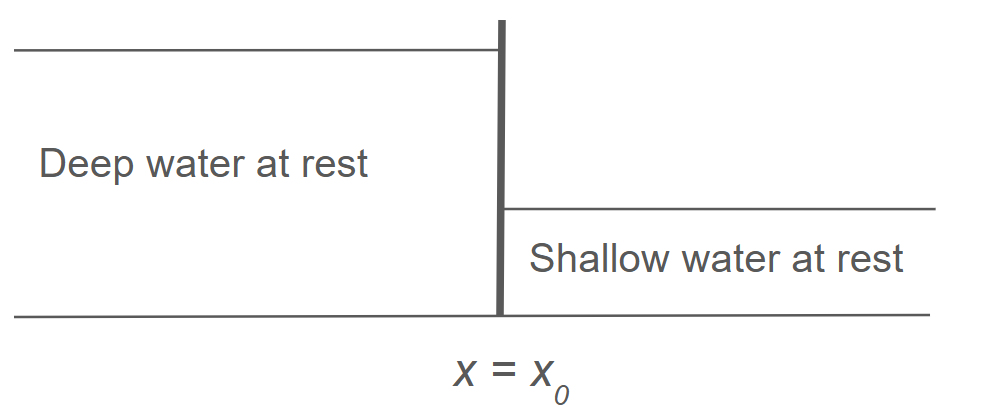
\includegraphics[width=0.5\textwidth]{C:/Users/Matteo/Shallow-Water-Equations/figs/dam-break-problem.png}
    \caption{Initial conditions for the dam-break problem. An infinitely thin wall at $x=x_0$ divides two sections of water with different water levels.}\label{fig:dam-break-problem}
\end{figure}
We can use the shallow water equations to model the flow of water in the dam-break problem, approximately, if we assume that the wall collapses instantaneously at $t=0$ s.
In this project we solve both the dam-break problem and cases of the Riemann problem, where the inital fluid velocity is nonzero.
The results are presented in \autoref{ch:numerical_results}.

\subsection{Solving the Riemann problem exactly by wave decomposition}
To get a better understanding of the flow in shallow water, we provide some very short background information about the wave structures in the solution of the Riemann problem.
In general, the wave structure in the solution of the Riemann problem~\eqref{eq:Riemann_problem} consists of three wave families separating four regions.
The wave families are denoted $W_1, W_2, W_3$ and the regions are the spaces between the wave families, denoted by $R_0, R_1, R_2$ and $R_3$.
The wave structure is illustrated in \autoref{fig:riemann_sol_general}.
\begin{figure}[H]
    \centering
    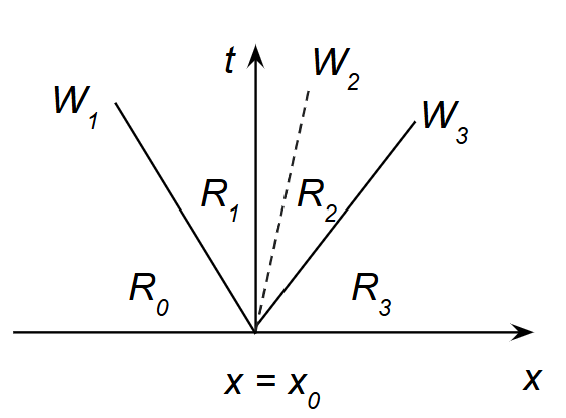
\includegraphics[width=0.5\textwidth]{C:/Users/Matteo/Shallow-Water-Equations/figs/riemann_sol_general.png}
    \caption{General wave structure in the solution of the Riemann problem.}\label{fig:riemann_sol_general}
\end{figure}
From \autoref{fig:riemann_sol_general} we see how the solution consists of three waves.
The left and right waves are either shock waves or rarefaction waves, and correspond to the one-dimensional shallow water equations.
The middle wave arises from the $y-$momentum equation in~\eqref{eq:Riemann_problem} and is always a shear wave.
The region between the left and right wave is called the star region and is interesting, since we do not know the solution in this region.
The star region is divided into two subregions $R_1$ and $R_2$.
The states in the regions are (from left to right) $U_L, U_{*L}, U_{*R}$ and $U_R$, where $U_L$ and $U_R$ are known, as these are the initial conditions.
The states $U_{*L}$ and $U_{*R}$ are in the regions $R_1$ and $R_2$, i.e., the star region and are unknown.
In the star region, we use $h_*$ to denote the water depth and $u_*$ to denote the velocity.
We can use $h_*$ to determine whether the left and right waves are shock waves or rarefaction waves.
Since we are considering the wet bed case, we can use the following characteristic:
\begin{equation*}
    \begin{cases}
        \text{The left wave is a shock wave} & \text{if } h_* > h_L, \\
        \text{The left wave is a rarefaction wave} & \text{if } h_* \leq h_L, \\        
    \end{cases} 
\end{equation*}
and similarly for the right wave:
\begin{equation*}
    \begin{cases}
        \text{The right wave is a shock wave} & \text{if } h_* > h_R, \\
        \text{The right wave is a rarefaction wave} & \text{if } h_* \leq h_R. \\        
    \end{cases} 
\end{equation*}
A shock wave is characterized by a discontinuity in the solution.
On each side of the shock wave, the water properties, such as height and velocity, differ significantly.
In contrast, a rarefaction wave represents a smooth transition in the solution.
The water height and velocity change gradually across the wave, and the properties are more similar on each side of the wave, without the sharp edges seen in a shock wave.
In the solution of the Riemann problem~\eqref{eq:Riemann_problem} there are four possible wave patterns outcomes, which are combinations of shock waves and rarefaction waves.
The left and right waves are either shock waves or rarefaction waves.
The four possible wave patterns are as follows:
\begin{enumerate}[label= (\alph*)]
    \item Left rarefaction, right shock,
    \item Left shock, right rarefaction,
    \item Both left and right rarefaction,
    \item Both left and right shock.
\end{enumerate}
In the example of the dam-break problem, with inital conditions as in Figure~\ref{fig:dam-break-problem}, the solution consists of a left rarefaction wave and a right shock wave.
This means that the shock wave moves to the right and is characterized by a discontinuity in the solution and a high speed.
Whereas, the rarefaction wave moves to the left and is characterized by a more smooth transition in the solution and a lower speed.
The Riemann solver computes the flux across the interface between two cells, considering the left and right states.
The numerical fluxes calculated by the Riemann solver allow for the determination of the state in the star region, which represents the solution at the interface between the two regions.
This is essential for determining whether the wave is a shock or a rarefaction wave, ensuring both the stability and accuracy of the numerical scheme.
In summary, Riemann solvers and numerical fluxes are crucial for solving for the states in the star region, which are then used to update the solution at each timestep.

%Hence the structure of the solution in general is shown in the figure below.
%From the figure we see that the solution consists of three waves, a left wave, a middle wave and a right wave, which together seperate four regions, described by the vector
%\begin{align*}
%\mathbf{W} = \begin{bmatrix}
%    h \\ hu \\ hv
%    \end{bmatrix}.
%\end{align*}
%The four regions are describes by $\mathbf{W}_L$ (left data), $\mathbf{W}_R$ (right data), $\mathbf{W}_{*L}$ and $\mathbf{W}_{*R}$, which both denote star region data.
%We are interested in the star region data, since these are the unknowns.
%Based on the given initial conditions, we must determine the types of waves.
%Second, it is known that across the left and right waves, both $h$ and $u$ change but $v$ remains constant.
%Whereas across the middle wave, $v$ changes but $h$ and $u$ remain constant.
%That is, $h$ and $u$ remain constant in the star region.
%Thus the water depth and particle velocity are constant in the star region and are denoted by $h_*$ and $u_*$, respectively.

%The exact Riemann solver is a method that solves the Riemann problem exactly, and it is based on the solution of the Riemann problem~\eqref{eq:Riemann_problem}.
%There exist exact Riemann solvers which are very efficient and leads to Gudonov methods, that are only slightly more expensive than those based on approximate Riemann solvers~\cite{Toro2001-Shock}.

%But for now, we will consider the case where the solution consists of a single non-trivial wave and all other waves are assumed to have zero strenght.
%This is enough to solve the Riemann problem as it is always possible to solve the Riemann problem by considering one wave at a time.
%We denote the constant values of the water depth and particle velocity in the star region by $h_*$ and $u_*$, respectively.




\subsection{Implementation of the FVM in 1D}
The code to solve the SWE in 1D using FVM is based on the Godunov scheme with the exact Riemann solver.
The exact solution of the Riemann problem is found by using the Riemann invariants and the Rankine-Hugoniot conditions~\cite{trento_course}.

The true solution is found by solving the Riemann problem exact, with 5000 cells, and distinguishing between the wetbed or drybed case, and also identifying the shock and rarefaction waves.


\subsection{Godunov's Method}
We consider the Godunov Upwind method, which is a first-order accurate metod to solve non-linear systems of hyperbolic conservation laws~\cite{Toro2024}.
Godunov's method is a fundamental starting point.
In the method we solve the non-linear Riemann problem at each cell interface. 

Consider the initial-boundary value problem (IBVP) for a system of $N$ nonlinear hyperbolic conservation (balance?) laws     
\begin{equation}\label{eq:IBVP_system}
    \begin{cases}
    \text{PDEs: }    &\mathbf{U}_t + \mathbf{F(U)}_x = \mathbf{S(U)}, \quad x \in [a, b], \quad t > 0, \\
    \text{ICs: }    &\mathbf{U}(x,0) = \mathbf{U}^{(0)}(x), \quad x \in [a,b], \\
    \text{BCs: }    &\mathbf{U}(a,t) = \mathbf{B}_{L}(t), \quad \mathbf{U}(b,t) = \mathbf{B}_{R}(t), \quad t \geq 0.
    \end{cases}
\end{equation}
The vectors $\mathbf{B}_L (t)$ and $\mathbf{B}_R (t)$ denote the boundary conditions at the left and right boundaries, respectively.
The Godunov Upwind method in conservative form~\eqref{eq:explicit_conservative_1D_SWE} solves the IBVP~\eqref{eq:IBVP_system}.


\subsection{Implementation of the FVM in 2D}


\subsection{Data generation}










